\chapter{Introduction}

\fwap is a modern domain specific programming language (DSL) that has an imperative structure, with parallel execution support and higher order functions \cite{exercise}. 

The developing team working at project was structured as an Agile one, with three collaborating, self-organizing groups working to the implementation of
\begin{enumerate}
	\item the parser/tokenizer module (with Coco/R and C\texttt{\#})
	\item the interpreter (written in C\texttt{\#})
	\item the \fsharp compiler (also written in C\texttt{\#})
\end{enumerate}
respectively. 

Eventually, the whole group worked together to the server performing the distributed tasks and to the online version of the compiler and the interpreter, available on GitHub \cite{proj}.
\begin{center}
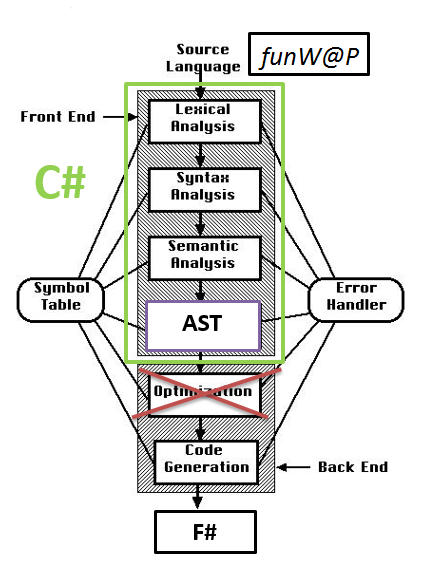
\includegraphics[height=12cm]{images/projectStructure}\\
\end{center}
